%%%%%%%%%%%%%%%%%%%%%%%%%%%%%%%%%%%%%%%%%
% Beamer Presentation
% LaTeX Template
% Version 1.0 (10/11/12)
%
% This template has been downloaded from:
% http://www.LaTeXTemplates.com
%
% License:
% CC BY-NC-SA 3.0 (http://creativecommons.org/licenses/by-nc-sa/3.0/)
%
%%%%%%%%%%%%%%%%%%%%%%%%%%%%%%%%%%%%%%%%%

%----------------------------------------------------------------------------------------
%	PACKAGES AND THEMES
%----------------------------------------------------------------------------------------

\documentclass[aspectratio=1610]{beamer}

\mode<presentation> {

% The Beamer class comes with a number of default slide themes
% which change the colors and layouts of slides. Below this is a list
% of all the themes, uncomment each in turn to see what they look like.

%\usetheme{default}
%\usetheme{AnnArbor}
%\usetheme{Antibes}
%\usetheme{Bergen}
%\usetheme{Berkeley}
%\usetheme{Berlin}
%\usetheme{Boadilla}
%\usetheme{CambridgeUS}
%\usetheme{Copenhagen}
%\usetheme{Darmstadt}
\usetheme{Dresden}
%\usetheme{Frankfurt}
%\usetheme{Goettingen}
%\usetheme{Hannover}
%\usetheme{Ilmenau}
%\usetheme{JuanLesPins}
%\usetheme{Luebeck}
%\usetheme{Madrid}
%\usetheme{Malmoe}
%\usetheme{Marburg}
%\usetheme{Montpellier}
%\usetheme{PaloAlto}
%\usetheme{Pittsburgh}
%\usetheme{Rochester}
%\usetheme{Singapore}
%\usetheme{Szeged}
%\usetheme{Warsaw}

% As well as themes, the Beamer class has a number of color themes
% for any slide theme. Uncomment each of these in turn to see how it
% changes the colors of your current slide theme.

%\usecolortheme{albatross}
%\usecolortheme{beaver}
%\usecolortheme{beetle}
%\usecolortheme{crane}
\usecolortheme{dolphin}
%\usecolortheme{dove}
%\usecolortheme{fly}
%\usecolortheme{lily}
%\usecolortheme{orchid}
%\usecolortheme{rose}
%\usecolortheme{seagull}
%\usecolortheme{seahorse}
%\usecolortheme{whale}
%\usecolortheme{wolverine}

%\setbeamertemplate{footline} % To remove the footer line in all slides uncomment this line
\setbeamertemplate{footline}[page number] % To replace the footer line in all slides with a simple slide count uncomment this line

\setbeamertemplate{navigation symbols}{} % To remove the navigation symbols from the bottom of all slides uncomment this line

\setbeamertemplate{bibliography item}{[\theenumiv]}

\setbeamertemplate{frametitle}[default][center]

\setbeamertemplate{caption}[numbered]

\setbeamertemplate{navigation symbols}{}

%---------------------------Picture Covering Full Slide---------------------------

\newif\ifsidebartheme
\sidebarthemetrue

\newdimen\contentheight
\newdimen\contentwidth
\newdimen\contentleft
\newdimen\contentbottom
\makeatletter
\newcommand*{\calculatespace}{%
\contentheight=\paperheight%
\ifx\beamer@frametitle\@empty%
    \setbox\@tempboxa=\box\voidb@x%
  \else%
    \setbox\@tempboxa=\vbox{%
      \vbox{}%
      {\parskip0pt\usebeamertemplate***{frametitle}}%
    }%
    \ifsidebartheme%
      \advance\contentheight by-1em%
    \fi%
  \fi%
\advance\contentheight by-\ht\@tempboxa%
\advance\contentheight by-\dp\@tempboxa%
\advance\contentheight by-\beamer@frametopskip%
\ifbeamer@plainframe%
\contentbottom=0pt%
\else%
\advance\contentheight by-\headheight%
\advance\contentheight by\headdp%
\advance\contentheight by-\footheight%
\advance\contentheight by4pt%
\contentbottom=\footheight%
\advance\contentbottom by-4pt%
\fi%
\contentwidth=\paperwidth%
\ifbeamer@plainframe%
\contentleft=0pt%
\else%
\advance\contentwidth by-\beamer@rightsidebar%
\advance\contentwidth by-\beamer@leftsidebar\relax%
\contentleft=\beamer@leftsidebar%
\fi%
}
\makeatother
%---------------------------------------------------------------------------





}

\usepackage{graphicx} % Allows including images
\usepackage{booktabs} % Allows the use of \toprule, \midrule and \bottomrule in tables
\usepackage{comment}
\usepackage{tikz}
\usepackage[outercaption]{sidecap}
\usepackage{color}
\usepackage{pdfpages}
\usepackage{tikz}
\usepackage{listings}


%----------------------------------------------------------------------------------------
%	TITLE PAGE
%----------------------------------------------------------------------------------------

\title[]{Embedding Programming Languages : \\* \textsc{Prolog} in \textsc{Haskell}} % The short title appears at the bottom of every slide, the full title is only on the title page

\author{Mehul Solanki} % Your name
\institute[UNBC] % Your institution as it will appear on the bottom of every slide, may be shorthand to save space
{
University of Northern British Columbia \\ % Your institution for the title page
\medskip
\textit{solanki@unbc.ca} % Your email address
\\ 230108015
}
\date{\today} % Date, can be changed to a custom date

\newcommand\mytext{\normalsize{Mehul Solanki}}

%\makeatother
%\setbeamertemplate{footline}
%{%
%  \leavevmode%
% \hbox{\begin{beamercolorbox}[wd=.5\paperwidth,ht=2.5ex,dp=1.125ex,leftskip=.3cm,rightskip=.3cm]{author in head/foot}%
 % \mytext
%  \end{beamercolorbox}%
%  \begin{beamercolorbox}[wd=.5\paperwidth,ht=2.5ex,dp=1.125ex,leftskip=.3cm,rightskip=.3cm plus1fil]{author in head/foot}%
%    \usebeamerfont{author in head/foot}\insertshortauthor\hfill\insertpagenumber
%  \end{beamercolorbox}}%
%  \vskip0pt%
%}
\makeatletter

%\author[MS]{Mehul Solanki}

\usetikzlibrary{trees}
\tikzset{hide on/.code={\only<#1>{\color{white}}}}

\begin{document}

\begin{frame}
\titlepage % Print the title page as the first slide
\end{frame}

%\begin{frame}
%\frametitle{Overview} % Table of contents slide, comment this block out to remove it
%\tableofcontents % Throughout your presentation, if you choose to use \section{} and \subsection{} commands, these will automatically be printed on this slide as an overview of your presentation
%\end{frame}

%----------------------------------------------------------------------------------------
%	PRESENTATION SLIDES
%----------------------------------------------------------------------------------------

%------------------------------------------------
%\section{Programming Languages} % Sections can be created in order to organize your presentation into discrete blocks, all sections and subsections are automatically printed in the table of contents as an overview of the talk
%------------------------------------------------
%\subsection{Subsection Example} % A subsection can be created just before a set of slides with a common theme to further break down your presentation into chunks
\begin{comment}
\begin{frame}
\frametitle{Programming Languages}

A programming language is an artificial language designed to communicate instructions to a machine, particularly a computer \cite{proglangwiki}.
\\*For example, C, Java.
\end{frame}
\end{comment}
%-------------------------------------------------

\begin{frame}
\frametitle{Programming Languages}
  \begin{columns}[T]
    \begin{column}{.4\textwidth}
     \begin{block}{}
A programming language is an artificial language designed to communicate instructions to a machine, particularly a computer \cite{proglangwiki}.
\\*For example, \textsc{C, Java}.
    \end{block}
    \end{column}
    \begin{column}{.6\textwidth}
    \begin{block}{}
% Your image included here
\begin{figure}
    
\includegraphics[width=1.1\textwidth]{progLanguages.jpg}
    
    \caption{The Universe of Programming Languages \cite{proglanguniv}}
 \end{figure}   
    \end{block}
    \end{column}
  \end{columns}
\end{frame}


%------------------------------------------------
\begin{comment}
\begin{frame}
\frametitle{Programming Paradigms}
A programming paradigm is a fundamental style of computer programming, a way of building the structure and elements of computer programs \cite{progparawiki}.
\\*For example, Object Oriented Programming.
\end{frame}
\end{comment}

\begin{frame}
\frametitle{Programming Language Paradigms}
  \begin{columns}[T]
    \begin{column}{.4\textwidth}
     \begin{block}{}
A programming paradigm is a fundamental style of computer programming, a way of building the structure and elements of computer programs \cite{progparawiki}.
\\*For example, Object Oriented Programming.
    \end{block}
    \end{column}
    \begin{column}{.6\textwidth}
    \begin{block}{}
% Your image included here
\begin{figure}
    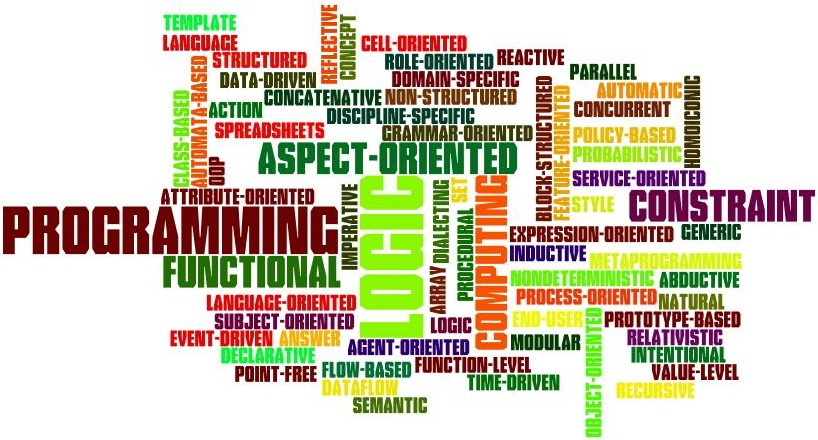
\includegraphics[width=1.1\textwidth]{programminglanguageparadigms.jpg} 
    \caption{Programming Paradigms \cite{progparawiki, progparawordle}}
 \end{figure}   
    \end{block}
    \end{column}
  \end{columns}
\end{frame}


%------------------------------------------------
\begin{comment}
\begin{frame}
\frametitle{Classification}
Programming languages are classified into paradigms depending on their characteristics and features. 
\\*For example, Java is an Object Oriented Programming Language \cite{javaintro}.     
\end{frame}
\end{comment}

\begin{frame}
\frametitle{Classification}
  \begin{columns}[T]
    \begin{column}{.5\textwidth}
     \begin{block}{}
Programming languages are classified into paradigms depending on their characteristics and features. 
\\*For example, \textsc{Java} is an Object Oriented Programming Language \cite{javaintro}.
    \end{block}
    \end{column}
    \begin{column}{.5\textwidth}
    \begin{block}{}
% Your image included here
\begin{figure}
    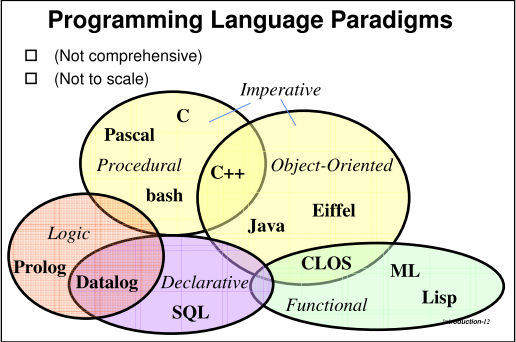
\includegraphics[width=\textwidth]{classification.png} 
    \caption{Classification of Programming Languages \cite{progparaclass}}
 \end{figure}   
    \end{block}
    \end{column}
  \end{columns}
\end{frame}

%------------------------------------------------
\begin{comment}
\begin{frame}
\frametitle{Logic programming}
In logic programming, a program consists of a collection of statements ex-pressed as formulas in symbolic logic. There are rules of inference from logic that allow a new formula to be derived from old ones, with the guarantee that if the old formulas are true, so is the new one \cite{spivey1996introduction}.
\\*For example, Prolog.
\end{frame}
\end{comment}

\begin{frame}
\frametitle{Logic Programming}
  \begin{columns}[T]
    \begin{column}{.5\textwidth}
     \begin{block}{}
In logic programming, a program consists of a collection of statements ex-pressed as formulas in symbolic logic. There are rules of inference from logic that allow a new formula to be derived from old ones, with the guarantee that if the old formulas are true, so is the new one \cite{spivey1996introduction}.
\\*For example, \textsc{Prolog}.
    \end{block}
    \end{column}
    \begin{column}{.5\textwidth}
    \begin{block}{}
% Your image included here
\begin{figure}
    
\includegraphics[width=\textwidth]{logicprogramming.jpg} 
    \caption{Logic Programming \cite{logicprogwordcloud}}
 \end{figure}   
    \end{block}
    \end{column}
  \end{columns}
\end{frame}

%------------------------------------------------
\begin{comment}
\begin{frame}
\frametitle{Prolog}
General purpose logic programming language with over 20 distributions \cite{prologwiki}. Prolog is a programming language borrowing its basic constructs from logic. A pure Prolog program is a logic program, in which an order is defined both clauses in the program and for goals in the body of the clause \cite{sterling1994art}.
\end{frame}
\end{comment}

\begin{frame}
\frametitle{\textsc{Prolog}}
  \begin{columns}[T]
    \begin{column}{.6\textwidth}
     \begin{block}{}
General purpose logic programming language with over 20 distributions \cite{prologwiki}. \textsc{Prolog} is a programming language borrowing its basic constructs from logic. A pure \textsc{Prolog} program is a logic program, in which an order is defined both clauses in the program and for goals in the body of the clause \cite{sterling1994art}.
    \end{block}
    \end{column}
    \begin{column}{.4\textwidth}
    \begin{block}{}
% Your image included here
\begin{figure}
    
\includegraphics[width=\textwidth]{swipl.png} 
    \caption{\textsc{SWI Prolog} Distribution \cite{swipl}}
 \end{figure}   
    \end{block}
    \end{column}
  \end{columns}
\end{frame}




%-------------------------------------------------




%------------------------------------------------
\begin{comment}
\begin{frame}
\frametitle{Functional Programming}
Programming in a functional language consists of building definitions and using the computer to evaluate expressions \cite{itfp}. 
\\*For example, Haskell.
\end{frame}
\end{comment}

\begin{frame}
\frametitle{Functional Programming}
  \begin{columns}[T]
    \begin{column}{.6\textwidth}
     \begin{block}{}
Programming in a functional language consists of building definitions and using the computer to evaluate expressions \cite{itfp}. 
\\*For example, \textsc{Haskell}.
    \end{block}
    \end{column}
    \begin{column}{.4\textwidth}
    \begin{block}{}
% Your image included here
\begin{figure}
    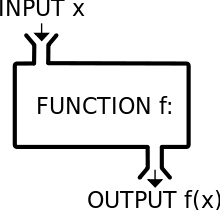
\includegraphics[width=\textwidth]{function-machine.jpeg} 
    \caption{Function \cite{funcmachine}}
 \end{figure}   
    \end{block}
    \end{column}
  \end{columns}
\end{frame}

%------------------------------------------------

\begin{comment}
\begin{frame}
\frametitle{Haskell}
Haskell is an advanced purely-functional programming language. In particular, it is a polymorphically statically typed, lazy, purely functional language \cite{haskellorg}.
\end{frame}
\end{comment}

\begin{frame}
\frametitle{\textsc{Haskell}}
  \begin{columns}[T]
    \begin{column}{.7\textwidth}
     \begin{block}{}
\textsc{Haskell} is an advanced purely-functional programming language. In particular, it is a polymorphically statically typed, lazy, purely functional language \cite{haskellorg}.
    \end{block}
    \end{column}
    \begin{column}{.3\textwidth}
    \begin{block}{}
% Your image included here
\begin{figure}
    
\includegraphics[width=\textwidth]{haskelllogo.jpg} 
    \caption{\textsc{Haskell} Programming Language \cite{haskelllogo}}
 \end{figure}   
    \end{block}
    \end{column}
  \end{columns}
\end{frame}



%------------------------------------------------

\begin{comment}
\begin{frame}
\frametitle{Alternate Classification}
A programming language inherits features from a number of paradigms rather than belonging to a single paradigm\cite{krishnamurthi2008teaching}.
\end{frame}
\end{comment}




\begin{frame}
\frametitle{Alternate Classification}
  \begin{columns}[T]
    \begin{column}{.7\textwidth}
     \begin{block}{}
A programming language inherits features from a number of paradigms rather than belonging to a single paradigm\cite{krishnamurthi2008teaching}.
    \end{block}
    \end{column}
    \begin{column}{.3\textwidth}
    \begin{block}{}
% Your image included here
\begin{figure}
    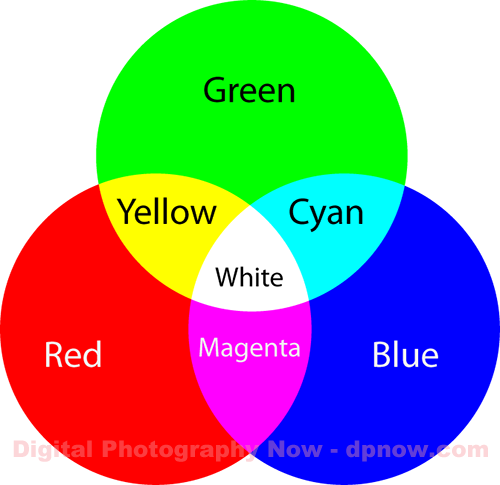
\includegraphics[width=\textwidth]{colourmixing2.png} 
    \caption{Mixing Colours \cite{colourmixing}}
 \end{figure}   
    \end{block}
    \end{column}
  \end{columns}
\end{frame}

%---------------------------------------------
%\begin{comment}
   \begin{frame}{Alternate Classification}
    \frametitle{Alternate Classification}

   \begin{figure}
        \begin{tikzpicture}[remember picture,overlay]
            \node[at=(current page.center)] {
                \includegraphics[width=\paperwidth]{programming-paradigms_label2.png}
            };
 %           \node[below=cm] at (current bounding box.base) {Programming Paradigms and Languages \cite{}};
        \end{tikzpicture}
   \caption{Programming Paradigms and Languages \cite{proglanggraph} \href{http://zoom.it/6rJp}{\beamergotobutton{Link}}}
         \end{figure}
   
     \end{frame}
%    \end{comment}
 
%---------------------------------
%----------------------------

\begin{comment}
\setbeamertemplate{background canvas}{%
\calculatespace%
\begin{pgfpicture}
    \pgfpathrectangle{\pgfpointorigin}{\pgfpoint{\paperwidth}{\paperheight}}
    \pgftext[at=\pgfpoint{\contentleft+0.5\contentwidth}{\contentbottom+0.5\contentheight}]{
\includegraphics[width=\contentwidth,height=\contentheight]{swipl.png}}

\end{pgfpicture}
}

\begin{frame}
\begin{figure}

\includegraphics[width=\contentwidth,height=\contentheight]{swipl.png}
\end{figure}
\end{frame}
\end{comment}




\begin{comment}
%---------------------------------------------

\begin{frame}
\framezoom<1><2>[border=4](6.8cm,1.2cm)(1.4cm,1.5cm)
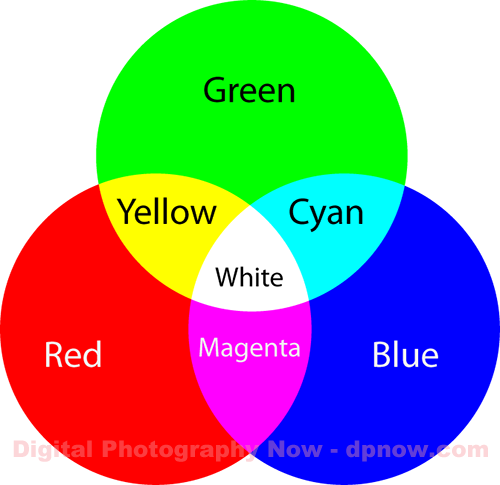
\includegraphics[height=\textheight,width=\textwidth,keepaspectratio]{colourmixing2.png}
\end{frame}

%-----------------------------------------------

\begin{frame}<1>[label=zooms]
\frametitle<1>{The \TeX{} logo}
\frametitle<2>{The letter ``T''}
\frametitle<3>{The letter ``E''}
\frametitle<4>{The letter ``X''}
\framezoom<1><2>[border](0.1cm,0cm)(3.6cm,4cm)
\framezoom<1><3>[border](3.4cm,1.2cm)(2.7cm,4.1cm)
\framezoom<1><4>[border](5.7cm,0cm)(3.7cm,4cm)
{\scalebox{15}{\TeX}\\}
\end{frame}

\begin{frame}{Next Slide}
    next slide
\end{frame}

\againframe<2->[noframenumbering]{zooms}
\end{comment}
%-----------------------------------------------

\begin{comment}
\begin{frame}
\frametitle{Programmer's Dilema}
\begin{description}
\item[$\bullet$] Number of languages.
\end{description}
\end{frame}
\end{comment}


\begin{frame}
\frametitle{Programmer's Dilemma}
  \begin{columns}[T]
    \begin{column}{.2\textwidth}
     \begin{block}{}
Increasing number of programming languages.
\href{http://zoom.it/5WN3}{\beamergotobutton{Link}}
    \end{block}
    \end{column}
    \begin{column}{0.8\textwidth}
    \begin{block}{}
% Your image included here
\begin{figure}
    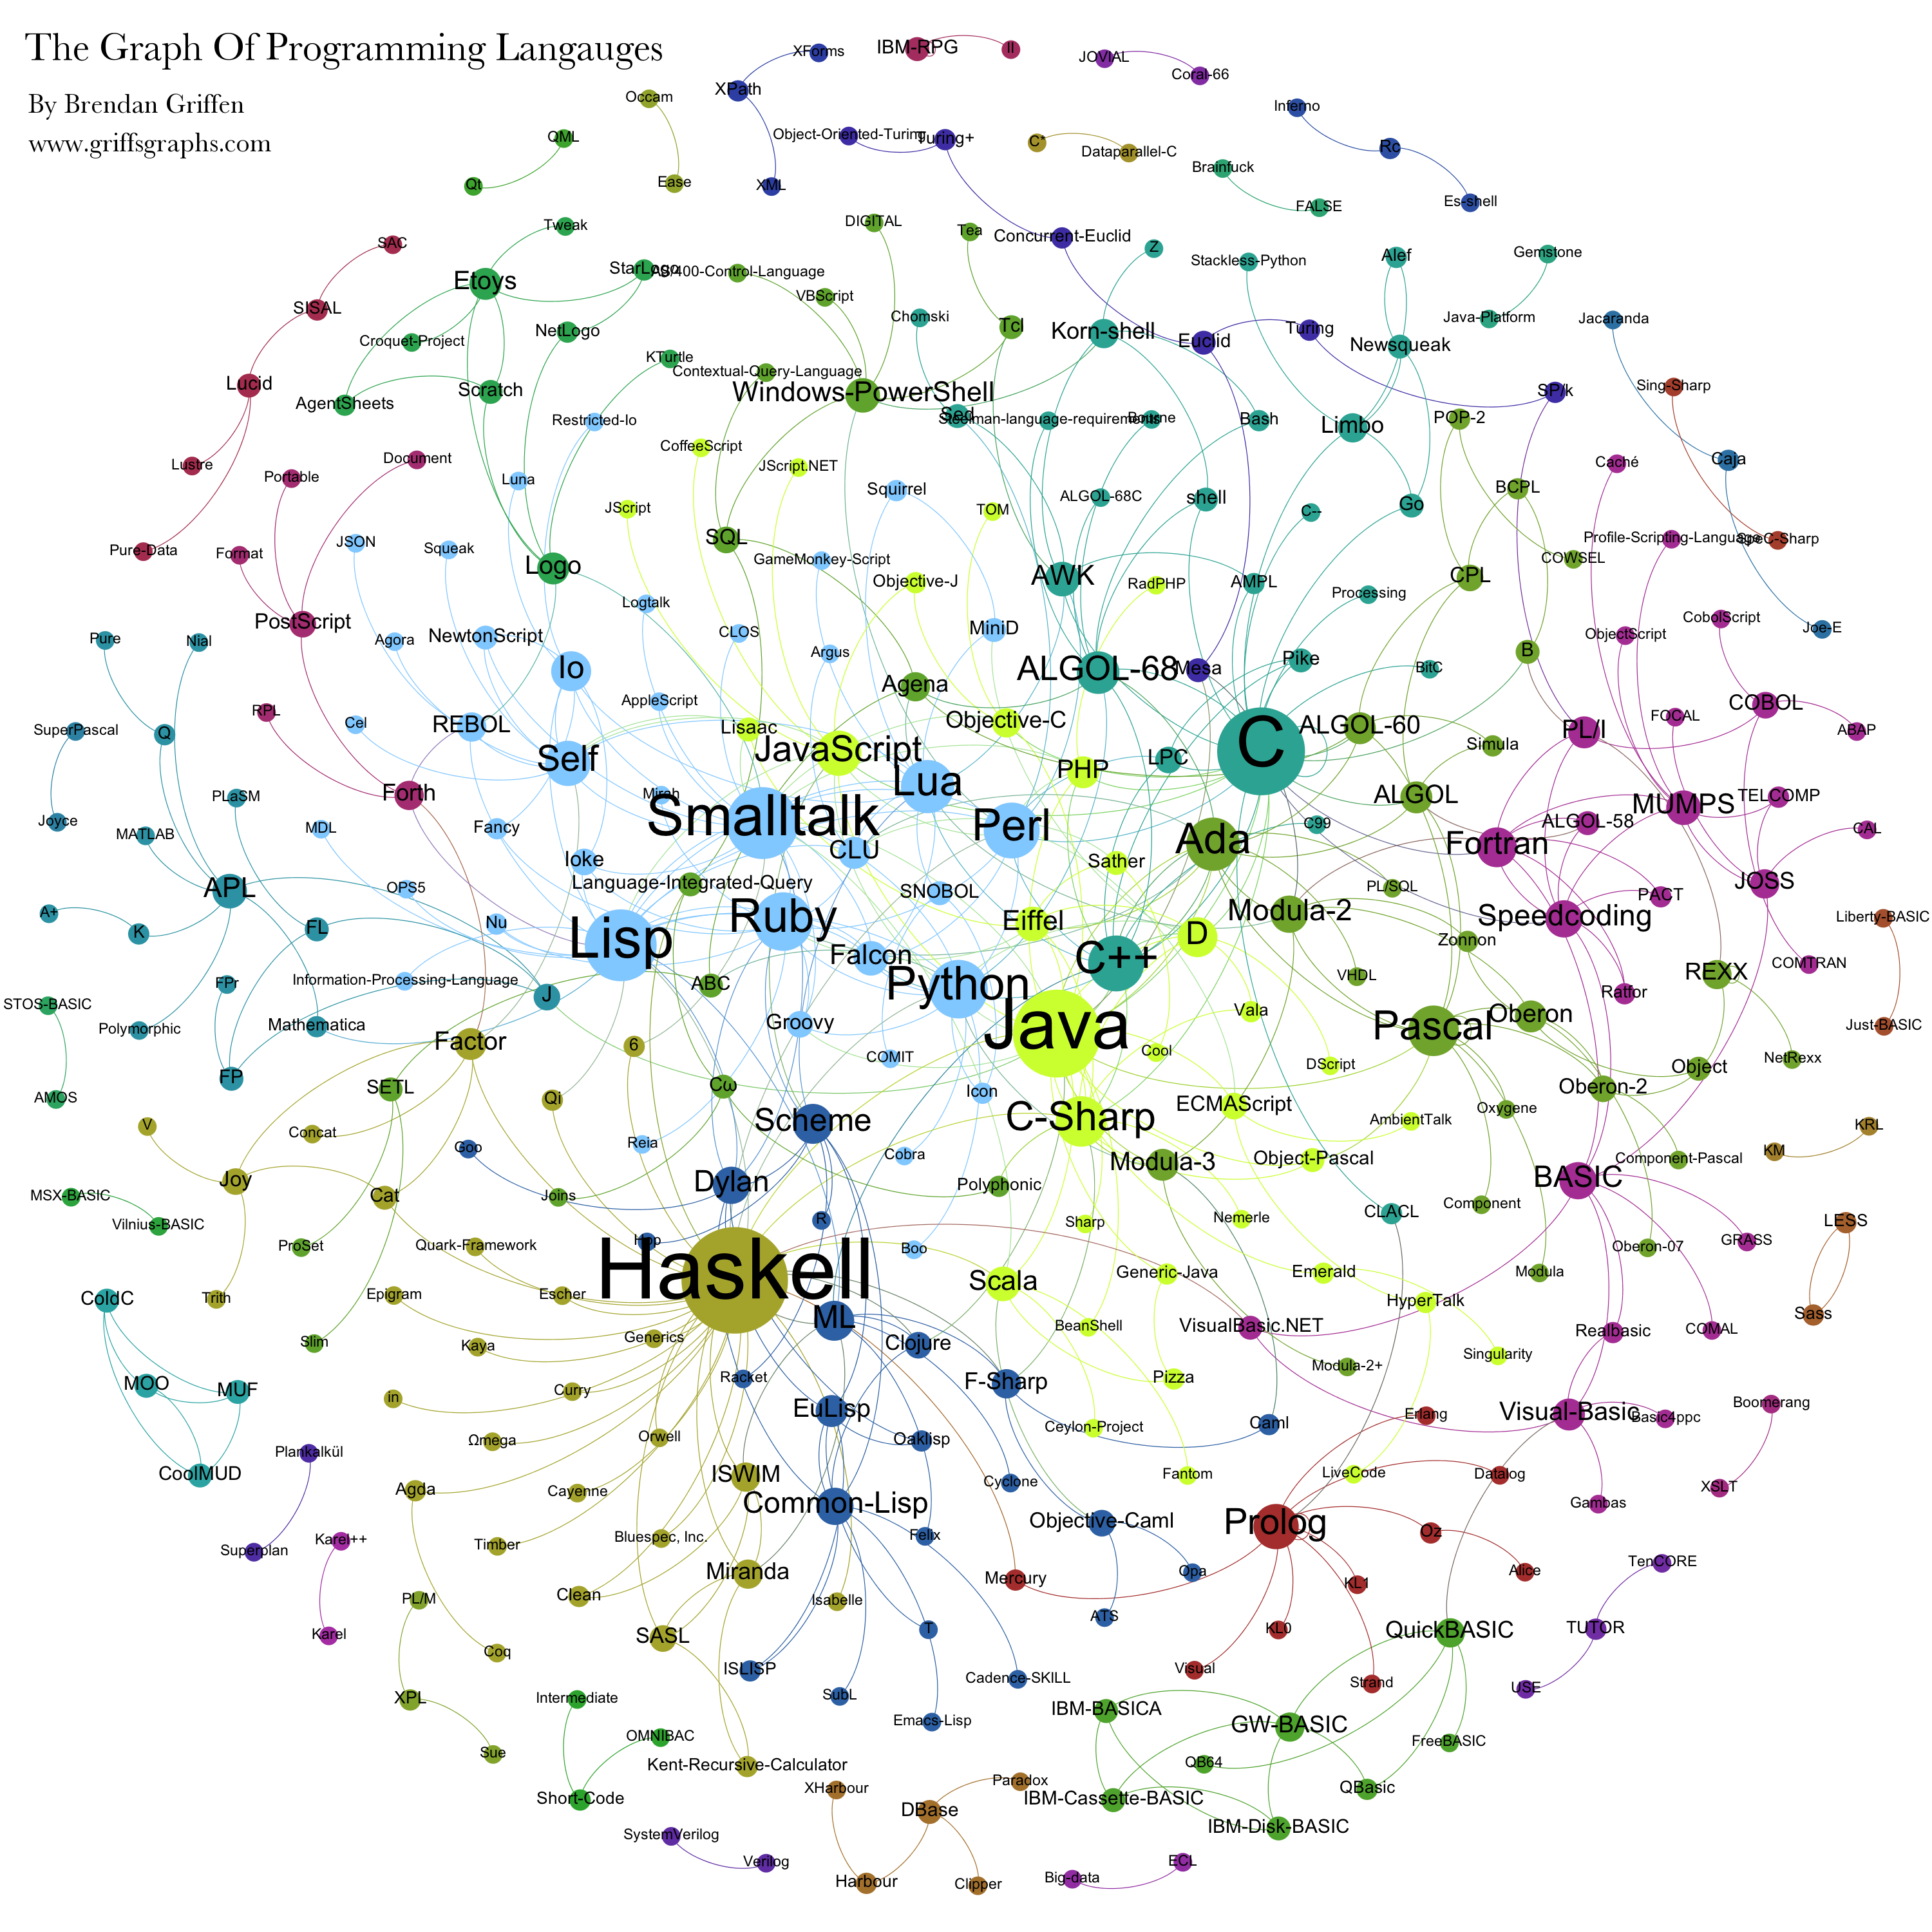
\includegraphics[height = 0.6\textwidth, width=0.6\textwidth]{programming-languages_2.png} 
    \caption{The Graph of programming Languages\cite{proglanggraph}}
 \end{figure}   
    \end{block}
    \end{column}
  \end{columns}
\end{frame}

%-----------------------------------------------
\begin{frame}
 \frametitle{General versus Special}
 \begin{columns}[T]
  \begin{column}{0.5\textwidth}
   \begin{block}{General Purpose Language}
    \textcolor{green}{Broad scope} but \textcolor{red}{problem needs to be moulded according to the capability of the language} \cite{gplwiki}.
   \end{block}
  \end{column}

  \begin{column}{0.5\textwidth}
   \begin{block}{Special Purpose Language}
    \textcolor{red}{Limited scope} but \textcolor{green}{easier to express the problem as the suitable capabilities are readily available} \cite{splwiki}. 
   \end{block}
  \end{column}
 \end{columns}
\end{frame}


%------------------------------------------------

\begin{frame}
\frametitle{Size Concern}
Software applications have and are continuing to grow in size. On an average a software applications has hundereds of thousands of lines of code \cite{codebases}. \href{http://www.informationisbeautiful.net/visualizations/million-lines-of-code/}{\beamergotobutton{Link}}

For example, the Windows application Paint has over 150,000 lines of code \cite{paintwiki}. 

\end{frame}

%----------------------------------------------------
\begin{comment}
\begin{frame}

\href{http://tex.stackexchange.com/q/20800/5701}{\beamergotobutton{Link}}

\end{frame}
\end{comment}

%------------------------------------------------
\begin{frame}
\frametitle{Problems with respect to \textsc{Prolog}}
Lacks basic features such as modules \cite{prologwiki}.

Not suitable for large programs, \cite{somogyi1995logic}, always under 100,000 lines of code \cite{prolog1000db}.
 
Fading usage in the industry \cite{website:prolog-death, website:prolog-killer, website:prolog-steam}. 
\end{frame}


%------------------------------------------------

\begin{frame}
\frametitle{As an Exercise}

\begin{columns}[T]
  \begin{column}{0.5\textwidth}
   \begin{block}
	
	  Conflicting characteristics.
		
    Principle differences. 
		
		
   \end{block}
  \end{column}

  \begin{column}{0.5\textwidth}
	\begin{figure}
   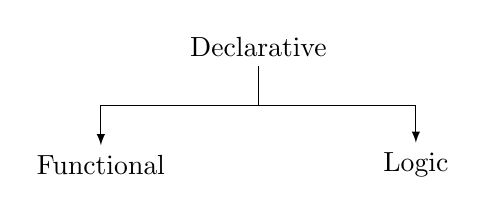
\begin{tikzpicture}[
  level 1/.style={sibling distance=40mm},
  edge from parent/.style={->,draw},
  >=latex]
%   \only<4>{} % Force beamer to show the correct amount of slides
    \node {Declarative}
    [edge from parent fork down]
    child {node {Functional}}
    child {node {Logic}
    };
\end{tikzpicture}
\caption{Declarative Programming Paradigms \cite{declarprogwiki}}
\end{figure}
  \end{column}
 \end{columns}
\end{frame}


\begin{frame}[fragile]
\frametitle{Comparison}
\center
\begin{table}
\begin{tabular}{|c|c|c|}
\hline
\textbf{\textcolor{blue}{Factor}} & \textbf{\textcolor{red}{\textsc{Haskell}}} & \textbf{\textcolor{green}{\textsc{Prolog}}} \\
\hline
\textcolor{blue}{Evaluation} & \textcolor{red}{Lazy} & \textcolor{green}{Strict} \\
\hline
\textcolor{blue}{Type System} & \textcolor{red}{Strong} & \textcolor{green}{Weak} \\
\hline
\textcolor{blue}{Working} & \textcolor{red}{Pattern Matching} & \textcolor{green}{Unification} \\
\hline
\textcolor{blue}{Purity} & \textcolor{red}{Monadic / Pure} & \textcolor{green}{Ad-hoc} \\
\hline
\end{tabular}
\caption{\textsc{Haskell} \cite{haskellorg} versus \textsc{Prolog} \cite{prologwiki}}
\end{table}

For example, consider the following code,

\begin{table}
\begin{tabular}{|c|c|}
\hline

\textbf{Pattern Matching} & \textbf{Unification} \\

\hline
\begin{lstlisting}
let (x,y) = (1,2)
x = 1
y = 2
\end{lstlisting} &
\begin{lstlisting}
(X,2) = (1,Y).
X = 1.
Y = 2. 
\end{lstlisting} \\ 

\hline
\end{tabular}
\end{table}

\end{frame}

%----------------------------------------------

\begin{frame}
\frametitle{Bringing programming languages closer}

The language moulds itself according to the problem. 

\hspace{5mm}

Reduce the hassle of jumping between languages. 

\hspace{5mm}

Language helps the programmer. 

\end{frame}


%-------------------------------------------------


\begin{frame}
\frametitle{Embedding Languages}

Language within another language.

\begin{enumerate}
\item Foreign Function Interface (FFI)
 \\* A mechanism by which a program written in one programming language can make use of services written in another language \cite{ffiwiki}. 
\\* For example, \textsc{Haskell} provides a mechanism to embed \textsc{C} code in its programs \cite{ffihaskwiki}.

\item Library or Module Extension
\\* Replicate the features and characteristics of the target language into the host. 
\\* For example, LogLisp \cite{loglisp} is \textsc{Prolog} library for \textsc{Lisp}. 
\end{enumerate}

\end{frame}

%---------------------------------------------------

\begin{frame}
\frametitle{Merging Paradigms}
Combining different programming paradigms or programming styles in one environment or in one system \cite{jerinic1993perspective}.

\hspace{5mm}

The idea of a multi paradigm language is to provide a framework in which programmers can work in a variety of styles, freely
intermixing constructs from different paradigms \cite{progparawiki}.
\end{frame}

%------------------------------------------------

\begin{frame}
\frametitle{\textsc{Scala}}
\textsc{Scala} is an object functional programming language \cite{scalawiki}.   

\begin{table}%
\begin{tabular}{|c|c|}
\hline
\textbf{Functional} & \textbf{Object Oriented}  \\
\hline
 Currying & Classes\\
\hline
Pattern Matching & Objects\\ 
\hline 
Algebraic Data Types & Interfaces\\ 
\hline 
Lazy Evaluation & Java Interoperation\\ 
\hline
Tail Recursion & Inheritance\\ 
\hline 
Immutability & Mutability\\
\hline
Higher Order Functions & Dynamic Class Loading\\
\hline
\end{tabular}
\caption{\textsc{Scala} Features \cite{scalaproglang}}
\label{}
\end{table}

\end{frame}


%------------------------------------------------
\begin{frame}
\frametitle{SITREP}
\begin{enumerate}
	\item Libraries lack support for practical \textsc{Prolog} features.
	
	\item Few \textsc{Haskell} based hybrid languages.
	\\* For example, \textsc{Curry} \cite{curryproglang}, a functional logic programming language.  
	
	\item Literature lacks implementations.
	
	\item Not many \textsc{Prolog} environments for \textsc{Haskell}. 
	
	\item No usage of \textit{haskellian} features. 
\end{enumerate}
\end{frame}

%--------------------------
%----------------------------------------------

\begin{frame}
\frametitle{Practically speaking}
\begin{enumerate}
\item \textsc{Prolog} searches for solutions using depth first search (DFS) and may result in infinite search tree.
\\* The \textit{cut} operator limits the search. 
	
\item Handling interactions with other technologies.
\\* For example, input, output, databases among others.

\end{enumerate}
\end{frame}

%------------------------------------------------

%----------------------------------------------

\begin{frame}
\frametitle{Hybrid Approach}
\center
\begin{table}%
\begin{tabular}{|c|c|}
\hline
\textbf{Shallow Embedding} & \textbf{Deep Integration}\\
\hline
Translation & Working together\\
\hline
Replicate working & Merging of properties \\
\hline
Under utilization of host language features & Unnecessary baggage \\
\hline
\end{tabular}
\caption{Embedding versus Merging Paradigms}
\label{}
\end{table}

\vspace{2mm}

\textbf{Hybrid Approach}
\\*Integrate core language features and embed other characteristics.

\end{frame}

%------------------------------------------------

\begin{frame}
\frametitle{Proposed Work}
\begin{enumerate}
	\item Practical features.
	
	\item Database capabilities.
	
	\item Type support.
	
	\item Handling IO.
	
	\item Hybrid language features. 
\end{enumerate}
\end{frame}

%--------------------------------------------------
\begin{frame}
	\frametitle{Possible Outcomes}
	
\begin{enumerate}
\item Choosing a programming language made easier.

\item A complete \textsc{Prolog} library with support for practical features.

\item Theoretical Model for working with IO.

\item General Embedding Scheme.   
\end{enumerate}
\end{frame}


%------------------------------------------------

\begin{comment}

%------------------------------------------------


%------------------------------------------------
\begin{frame}
\frametitle{Bullet Points}
\begin{itemize}
\item Lorem ipsum dolor sit amet, consectetur adipiscing elit
\item Aliquam blandit faucibus nisi, sit amet dapibus enim tempus eu
\item Nulla commodo, erat quis gravida posuere, elit lacus lobortis est, quis porttitor odio mauris at libero
\item Nam cursus est eget velit posuere pellentesque
\item Vestibulum faucibus velit a augue condimentum quis convallis nulla gravida
\end{itemize}
\end{frame}

%------------------------------------------------

\begin{frame}
\frametitle{Blocks of Highlighted Text}
\begin{block}{Block 1}
Lorem ipsum dolor sit amet, consectetur adipiscing elit. Integer lectus nisl, ultricies in feugiat rutrum, porttitor sit amet augue. Aliquam ut tortor mauris. Sed volutpat ante purus, quis accumsan dolor.
\end{block}

\begin{block}{Block 2}
Pellentesque sed tellus purus. Class aptent taciti sociosqu ad litora torquent per conubia nostra, per inceptos himenaeos. Vestibulum quis magna at risus dictum tempor eu vitae velit.
\end{block}

\begin{block}{Block 3}
Suspendisse tincidunt sagittis gravida. Curabitur condimentum, enim sed venenatis rutrum, ipsum neque consectetur orci, sed blandit justo nisi ac lacus.
\end{block}
\end{frame}

%------------------------------------------------

\begin{frame}
\frametitle{Multiple Columns}
\begin{columns}[c] % The "c" option specifies centered vertical alignment while the "t" option is used for top vertical alignment

\column{.45\textwidth} % Left column and width
\textbf{Heading}
\begin{enumerate}
\item Statement
\item Explanation
\item Example
\end{enumerate}

\column{.5\textwidth} % Right column and width
Lorem ipsum dolor sit amet, consectetur adipiscing elit. Integer lectus nisl, ultricies in feugiat rutrum, porttitor sit amet augue. Aliquam ut tortor mauris. Sed volutpat ante purus, quis accumsan dolor.

\end{columns}
\end{frame}

%------------------------------------------------
%\section{Second Section}
%------------------------------------------------

\begin{frame}
\frametitle{Table}
\begin{table}
\begin{tabular}{l l l}
\toprule
\textbf{Treatments} & \textbf{Response 1} & \textbf{Response 2}\\
\midrule
Treatment 1 & 0.0003262 & 0.562 \\
Treatment 2 & 0.0015681 & 0.910 \\
Treatment 3 & 0.0009271 & 0.296 \\
\bottomrule
\end{tabular}
\caption{Table caption}
\end{table}
\end{frame}

%------------------------------------------------

\begin{frame}
\frametitle{Theorem}
\begin{theorem}[Mass--energy equivalence]
$E = mc^2$
\end{theorem}
\end{frame}

%------------------------------------------------

\begin{frame}[fragile] % Need to use the fragile option when verbatim is used in the slide
\frametitle{Verbatim}
\begin{example}[Theorem Slide Code]
\begin{verbatim}
\begin{frame}
\frametitle{Theorem}
\begin{theorem}[Mass--energy equivalence]
$E = mc^2$
\end{theorem}
\end{frame}\end{verbatim}
\end{example}
\end{frame}

%------------------------------------------------

\begin{frame}
\frametitle{Figure}
Uncomment the code on this slide to include your own image from the same directory as the template .TeX file.
%\begin{figure}
%\includegraphics[width=0.8\linewidth]{test}
%\end{figure}
\end{frame}

%------------------------------------------------

\begin{frame}[fragile] % Need to use the fragile option when verbatim is used in the slide
\frametitle{Citation}
An example of the \verb|\cite| command to cite within the presentation:\\~

This statement requires citation \cite{itfp}.
\end{frame}
\end{comment}
%------------------------------------------------

\begin{frame} [allowframebreaks]
\frametitle{References}
\footnotesize{
\begin{thebibliography}{9} % Beamer does not support BibTeX so references must be inserted manually as below

\bibitem{proglangwiki} Wikipedia (April 2014), Programming Languages, \url{http://en.wikipedia.org/wiki/Programming_language}.

\bibitem{progparawiki} Wikipedia (April 2014), Programming Paradigms, \url{http://en.wikipedia.org/wiki/Programming_paradigm}.

\bibitem{spivey1996introduction} Spivey, Michael (1996), \textit{An introduction to logic programming through Prolog}, \emph{ Prentice-Hall, Inc.} 

\bibitem{itfp} Richard Bird, Philip Wadler (1988), \textit{ Introduction to Functional Programming, 1st Edition},  \emph{ Prentice-Hall, Inc.}

\bibitem{krishnamurthi2008teaching} Krishnamurthi, Shriram (2008), Teaching programming languages in a post-linnaean age.

\bibitem{prologwiki} Wikipedia (April 2014), Prolog, \url{http://en.wikipedia.org/wiki/Prolog}.

\bibitem{sterling1994art} Sterling, Leon (1994), \textit{The art of Prolog: advanced programming techniques}, \emph{MIT press}.

\bibitem{haskellorg} The Haskell Programming Language (September 2013), Introduction to Haskell, \url{http://www.haskell.org/haskellwiki/Introduction}.

\bibitem{javaintro} The Java Programming Language (2014), Introduction to Java,
 \url{http://docs.oracle.com/javase/tutorial/getStarted/intro/definition.html}.

\bibitem{proglanguniv} LurnQ, Java compared with other languages, \url{http://lurnq.com/lesson/Java-Introduction-and-Comparison-with-Different-Programming-Languages}.

\bibitem{progpara} Pseudo Random, Software engineering in the Technion – semester 3, \url{http://epsilonvectorplusplus.wordpress.com/2011/03/30/software-engineering-in-the-technionsemester-3/}. 

\bibitem{progparaclass} US Study, Programming Languages, \url{http://www.ustudy.in/node/2834}. 

\bibitem{progparawordle} Wordle, Creating a word cloud, \url{http://www.wordle.net/}.

\bibitem{logicprogwordcloud} 123rf, Abstract word cloud for Logic, \url{http://www.123rf.com/photo_16414042_abstract-word-cloud-for-logic-with-related-tags-and-terms.html}.

\bibitem{swipl} SWI Prolog, \url{http://www.swi-prolog.org/}. 

\bibitem{funcmachine} Jan Kammerath (2012), The Joys of functional programming in Scala,  \url{http://www.kammerath.co.uk/The-Joys-of-functional-programming-in-Scala.html}.

\bibitem{haskelllogo} Wikimedia, Haskell Logo, \url{http://commons.wikimedia.org/wiki/File:Haskell-Logo.svg}.

\bibitem{colourmixing} Science by Mr.Macfarlane, Additive and Subtractive Colours, \url{http://mr.macfarlane.ws/index.php?/archives/14-Additive-and-Subtractive-Colours.html}.  

\bibitem{proglanggraph} Griff's Graphs, The Graph of Programming Languages, \url{http://griffsgraphs.com/2012/07/01/programming-languages-influences/}.

 \bibitem{gplwiki} Wikipedia, General Purpose Programming Languages, \url{http://en.wikipedia.org/wiki/General-purpose_programming_language}.
 
  \bibitem{splwiki}Wikipedia, Special Purpose Programming Languages, \url{http://en.wikipedia.org/wiki/Domain-specific_programming_language}.

   \bibitem{codebases}Information is beatiful (October 2013), Codebases, \url{http://www.informationisbeautiful.net/visualizations/million-lines-of-code/}.
   
   \bibitem{paintwiki} Wikipedia (March 2014), Paint.NET, \url{http://en.wikipedia.org/wiki/Paint.NET}.
   
   \bibitem{somogyi1995logic} Somogyi, Zoltan and Henderson, Fergus and Conway (1995), Thomas and O’Keefe, Richard, Logic programming for the real world, \textit{Proceedings of the ILPS} 83--94. 
 
    \bibitem{prolog1000db} Mark Kantrowitz (August 2012), The Prolog 1000 Datbase, \url{http://www.faqs.org/faqs/prolog/resource-guide/part1/section-9.html}.
    
    \bibitem{website:prolog-steam}Mark J Nelson (August 2010), Why did Prolog lose steam?, \url{http://www.kmjn.org/notes/prolog_lost_steam.html}.  
      
     \bibitem{website:prolog-death} Andre Vellino, (August 2010), Prolog's Death, \url{http://synthese.wordpress.com/2010/08/21/prologs-death/}.  

     \bibitem{website:prolog-killer} Maarten van Emden (August 2010), Who killed Prolog?, \url{http://vanemden.wordpress.com/2010/08/21/who-killed-prolog/}.      
    
		\bibitem{declarprogwiki} WIkipedia (March 2014), Declarative Programming, \url{http://en.wikipedia.org/wiki/Declarative_programming}.
		
		\bibitem{ffiwiki}Wikipedia (January 2014), Foreign function interface, \url{http://en.wikipedia.org/wiki/Foreign_function_interface}. 

    \bibitem{ffihaskwiki} Haskell Wiki (August 2013), Haskell Foreign Function Interface, \url {http://www.haskell.org/haskellwiki/FFI_Introduction}. 
		
		\bibitem{loglisp}J Alan Robinson and Ernest E Sibert (1982), Loglisp: Motivation, design, and implementation,\url{http://aitopics.org/sites/default/files/classic/Machine_Intelligence_10/MI10-Ch20-RobinsonSiberet.pdf}.
		
		\bibitem{jerinic1993perspective}Jerinic, Ljubomir and Obradovica, Trg D (1993), A Perspective on Combining Different Programming Paradigms.

		\bibitem{scalawiki} Wikipedia (April 2014), Scala Programming Language, \url{http://en.wikipedia.org/wiki/Scala_\%28programming_language\%29}.
	
		\bibitem{scalaproglang} The Scala Programming Language, What is Scala, \url{http://www.scala-lang.org/what-is-scala.html}.
		
		\bibitem{curryproglang} Curry Wiki, The Curry Programming Language, \url{http://www-ps.informatik.uni-kiel.de/currywiki/}.  
\end{thebibliography}
}
\end{frame}

%------------------------------------------------


%--------------------------------------------

\begin{frame}
\frametitle{The End}
\Huge{\centerline{Questions?}}
\end{frame}

%----------------------------------------------------------------------------------------

\end{document} 